\section{Mining Comparative Opinions}


%2) According to the word embedding, can we adopt better clustering methods?



For each pair of comparable technologies in the knowledge base, we analyze the Q\&A discussions in Stack Overflow to extract plausible comparative sentences by which Stack Overflow users express their opinions on the comparable technologies. 
\revise{Note that the comparison of comparable technologies may lie in one sentence, but also consecutive sentences.
So, we also take the context into consideration for comparison opinion extraction.}
%\wang{Sometimes users express their opinion in one simple comparative sentence, and sometimes they tend to compare technology pairs in two sentences respectively. Either way, we may obtain many comparative sentences for each pair of comparable technologies.}
Displaying all these sentences as a whole may make it difficult for developers to read and digest the comparison information.
Therefore, we measure the similarity among the comparative sentences, and then cluster them into several groups, each of which may identify a prominent aspect of technology comparison that users are concerned with.
%The extracted comparative sentences are clustered to reveal the prominent aspects that users are concerned with when comparing the two technologies.

\subsection{Extracting Comparative Sentences}
\label{sec:comparativeSentence}

There are three steps to extract comparative sentences of the two technologies.
We first carry out some preprocessing of the Stack Overflow post content.
Then we locate the sentences that contain the name of the two technologies, and further select the comparative sentences that satisfy a set of comparative sentence patterns.

\subsubsection{Preprocessing}
To extract trustworthy opinions about the comparison of technologies, we consider only answer posts with positive score points.
Then we split the textual content of such answer posts into individual sentences by punctuations like ``.'',  ``!'', ``?''.
We remove all sentences ended with question mark, as we want to extract facts instead of doubts. 
We further exclude sentences from question post, as most of them are assumptions or questions to ask.
We lowercase all sentences to make the sentence tokens consistent with the technology names because all tags are in lowercase. 
\begin{figure}
	\centering
	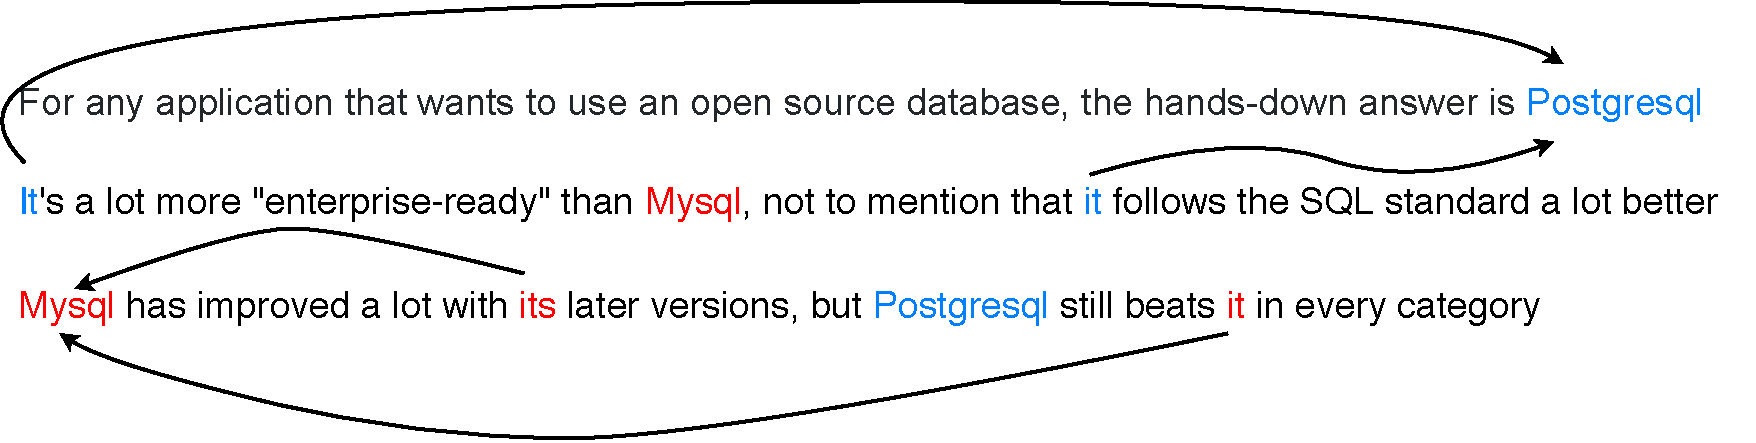
\includegraphics[width=0.47\textwidth]{figures/coreference.pdf}
	\vspace{1mm}
	\caption{An example of coreference resolution in comparative sentence.}
	\label{fig:coreference}
	\vspace{-3mm}
\end{figure}

\revise{Note that within the technical discussion in Stack Overflow, developers may adopt some pronoun like ``it'', ``that'', ``which'' to represent the technology.
For example, given the paragraph ``\textit{For any application that wants to use an open source database, the hands-down answer is postgresql. It's a lot more enterprise-ready than mysql, not ot mention that it follows the SQL standard a lot better. Mysql has improved a lot with its later versions, but Postgresql still beats it in every category.}'' as seen in Figure~\ref{fig:coreference}, the two ``it'' in the second sentence refers to ``postgresql'' in the first sentence. 
But with some cases, the reference may be too far from its source, leading to the negative influence to the location of comparative sentences. 
Therefore, we adopt the coreference resolution algorithm~\cite{clark2016deep} to recover the pronoun before locating comparative sentences.}

\revise{Conventionally, the coreference resolution is based on a set of manual-crafted rules by analyzing dependency tree of words in the sentence.
However, those rules may not be scalable, therefore, we adopt the state-of-the-art neural network based coreference method, named NeuralCoref\footnote{\url{https://github.com/huggingface/neuralcoref}}.
It feeds word embedding of potential words around each mention to two neural networks with one for giving score for finding a possible antecedent, and the other giving a score for a mention having no antecedent.
Given two scores, we compare them and pick the highest score to determine whether the mention has an antecedent and which word it is.}
  
\begin{comment}
\wang{We adopt the coreference method from NeuralCoref~\cite{}(site the github page?or medium page). The method extracts the mentions and potential antecedents by parsing sentences with spaCy parser~\cite{honnibal2015improved} first. Then it uses trained word embedding model, which was trained on the OntoNotes 5.0 dataset\cite{ralph2012ontonotes}, to tokenize pairs of mentions. The method includes the neural mention-ranking model\cite{clark2016deep}, which takes in the words vectors and some additional features(i.e. length of mentions, location of metnions...) as input. The input gets through four hidden layers of fully connected neural nets with rectified linear (ReLU) activation functions~\cite{nair2010rectified}, and the output links the the mention with its highest scored antecedent.  They apply the ranking model into two neural nets. One net is to give a score for each pair or mention and its possible antecedent, the other net is to give a score of the mention that doesn't have antecedents. Finally, given two scores, the method compares them and pick the highest score to determine whether the mention has an antecedent and which word it is. }
%\wang{We also use Coreference technique to preprocess sentences that contains tech pairs. The Coreference resolution can annotate sentence clusters and help us replace the pronoun with its corresponding subject, which should be helpful for us to locate and select comparative sentences in the following sections. Fig \ref{fig:coreference} shows that the Corefrerence reads that \textit{It} in the second sentence refers to the \textit{Postgresql} in the first sentece. So we further change the \textit{It} to \textit{Postgresql}, which makes it matches Pattern 2 for Single sentence.} 
\end{comment}



\subsubsection{Locating Candidate Sentences}
\revise{The sentences mentioning a pair of comparable technologies may contain the comparison opinion of them.
According to our observation, the comparison may occur in either one single sentence, or the contextual sentences.
Therefore, the candidate comparison sentences may be single sentences mentioning two comparable technologies, or the consecutive sentences with each of it containing one comparable technology respectively.
}

Note that using only the tag names is not enough.
As posts in Stack Overflow are informal discussions about programming-related issues, users often use alias to refer to the same technology.
Aliases of technologies can be abbreviations, synonyms and some frequent misspellings.
\revise{For example, there are several different alias of ``visual studio'' in many forms such as ``visual-studio'' (synonym), ``vs'' (abbreviation), and ``visual studion'' (misspelling) in the discussions.}
The presence of such aliases will lead to significant missing of comparative sentences, if we match technology mentions in a sentence with only tag names.
Chen et al.'s work~\cite{chen2019sethesaurus} builds a large thesaurus of morphological forms of software-specific terms, including abbreviations, synonyms and misspellings.
Table~\ref{tab:alias} shows some examples of technologies aliases in this thesaurus.
Based on this thesaurus, we find 7310 different alias for 3731 software technologies.
These aliases help to locate more candidate comparative sentences that mention certain technologies.

\begin{table}
	\scriptsize
	\center	
	\caption{Examples of alias}
	\vspace{-4mm}
	%\setlength{\tabcolsep}{0.3em}
    \setlength{\tabcolsep}{0.1em}
	\begin{tabular}{c c c}
		\hline
		\textbf{Tech term} & \textbf{Synonyms} & \textbf{Abbreviation} \\
		\hline
		photoshop & adobe\_photoshop, photoshops & ps \\
		dataframe & data-frame, pd.dataframe & df \\
		libgd &  gd\_library & gd \\		
        microsoft sql server & ms-sql, msql, ms\_sql & mssql \\
        		breadth-first search & breadth first search, breadth-first-search & bfs \\
				\hline
	\end{tabular}
	\vspace{-3mm}
	\label{tab:alias}
\end{table}

\subsubsection{Selecting Comparative Sentences}
%\textcolor{blue}{Not all sentences mentioning the two technologies are comparative sentences, for example, ... give an example ...}.
To identify comparative sentences from candidate sentences, we develop two sets of comparative sentence patterns: \revise{one for the single sentence and the other for contextual sentences.} 
Single sentence pattern is a sequence of POS tags. 
For example, the sequence of POS tags ``\textit{RBR JJ IN}'' is a pattern that consists of a comparative adverb (\textit{RBR}), an adjective (\textit{JJ}) and subsequently a preposition (\textit{IN}), such as "more efficient than", ``less friendly than'', etc. 
We extend the list of common POS tags to enhance the identification of comparative sentences.
More specifically, we create four comparative POS tags: \textit{CV} (comparative verbs, e.g. prefer, compare, beat), \textit{CIN} (comparative prepositions, e.g. than, over), \textit{NW} (negation words, e.g. wouldn't, doesn't ), and \textit{TECH} (technology reference, including the name and aliases of a technology, e.g. python, eclipse).

\begin{table*}
	\centering
	\caption{\revise{Patterns of comparative single sentences} \chen{1. Please change the examples 2. For each pattern, should we have both TECHs appearing in each pattern?}}
	\vspace{-3mm}
% 	\setlength{\tabcolsep}{0.1em}
\renewcommand{\arraystretch}{1.2}
	\textbf{Single sentence} 
	\begin{tabular}{l|l|l|l}
		\hline 
		\textbf{No.} & \textbf{Pattern} & \textbf{Sequence example} & \textbf{Original sentence} \\ \hline
		1 & \textit{TECH * VBZ * (JJR} $\lor$\textit{ RBR)} & innodb has 30 higher & InnoDB has 30\% higher performance than MyISAM on average. \\ \hline
		\multirow{2}{*}{2} & \multirow{2}{*}{\textit{((RBR JJ) } $\lor$\textit{ JJR) * CIN * TECH}} & faster than coalesce & Isnull is faster than coalesce. \\
		& & more complex than mysql & Triggers in postgresql have a syntax a bit more complex than mysql. \\ \hline
		3 & \textit{CV * CIN TECH} & recommend scylla over cassandra  & I would recommend scylla over cassandra. \\ \hline
		4 & \textit{CV VBG TECH} & recommend using html5lib & I strongly recommend using html5lib instead of beautifulsoup. \\
		\hline 
		%7 & \textit{CV TECH} & beat accurev & I have used svn, cvs,  clearcase but none of them can beat accurev's strengths\\ 
		%\vspace{1mm}	
	\end{tabular}
	
	\vspace{-3mm}
	\label{tab:patternSingle}
\end{table*}

%we find that comparative sentences can be represented by some specific comparative patterns.
Based on data observations of comparative sentences, we summarise four comparative patterns for single sentences as seen in Table~\ref{tab:patternSingle}.
To make the patterns more flexible, we use a wildcard character to represent a list of arbitrary words to match the pattern. 
For each sentence mentioning the two comparable technologies, we obtain its POS tags and check if it matches any one of four patterns.
If so, the sentence will be selected as a single comparative sentence.

\revise{For contextual candidate sentences, we develop three patterns for identifying comparative opinions in Table~\ref{tab:patternMultiple}. First, ... Second, ...}
\wang{The first two patterns are similar to the first two patterns in single sentence. Instead, those sentences tend to split the comparable technologies into each sentence respectfully. So we collect those sentences mentioned both of the comparable technology pairs, check if one of them match the POS tags pattern and the other sentence is using the second technology as a subject or an object, then we find a match.}
\chen{The first two patterns are further needed for discussion as there is some obvious flaw with it. For example, what if one sentence contain the pattern, the other sentence is not related to the pattern?}
\revise{The other pattern is that one contextual sentences is the affirmation (AFF) while the other is negation (NEG) with at least one comparable technology appears as the subject of one sentence.
For example, the prior sentence ``Cassini does not support HTTPs'' is the negation sentence, and the latter sentence ``However, you can use IIS to do this'' is the affirmation sentence, resulting in the comparison opinion that IIS can support the feature that is not owned by Cassini.}
\chen{How do we know one sentence is positive while the other is negative, and this example is not very good.}
\wang{In order to extract the \textit{AFF-NEG} pattern, We firstly create a list of negation words defined as ``\textit{NW}'' in POS tag. For each pair of sentences we check if either of them match the pattern ``\textit{TECH NW}'',so that we locate the negation sentence. Then, for the other sentence, we make sure it contains the other comparative tag and match the following one of the pattern:``\textit{TECH VB NN}'', ``\textit{TECH VB JJ}'', ``\textit{TECH VB RB}'', and ``\textit{VB TECH TO VB}''. All of which are making sure the other sentence is a affirmation sentence talking about the comparative tag. If the selected pair of sentences match the rules we talked above, we select them as \textit{AFF-NEG} pattern comparative sentences.  }

%\wang{During the process of exploring and observing real data, we find out that users also tend to describe a tech pair in two sentences, so we further develop the Contextual sentence. For two contextual sentences, if they contain two comparable technologies respectfully, and either of them match the first 2 patterns, we select them as contextual comparative sentence. For the \textit{POS-NEG} pattern, we collect sentences that contain comparable technologies but have different semantic statements, whereas one is positive the other is negative. Table~\ref{tab:pattern} shows these patterns and the corresponding examples of comparative sentences. s}
%According to these comparative patterns, we can determine whether a sentence is a comparative sentence or not. 


\begin{table*}
	\centering
	\caption{\revise{Patterns of comparative contextual sentences} \chen{1. The first two patterns need to be further discussed. 2. Please preserve the original style of the example}}
	\begin{tabular}{l|l|l|l}
		\hline 
		\textbf{No.} & \textbf{Pattern} & \textbf{Sequence example} & \textbf{Original sentence} \\ \hline
		\multirow{2}{*}{1} & \multirow{2}{*}{ \textit{TECH * VBZ * (JJR} $\lor$\textit{ RBR)}} & \multirow{2}{*}{triple des is generally better} & Triple des is generally better but there are some known theoretical attacks. \\ & & & If you have a choice of cipher you might want to look at aes instead. \\
		\hline
		\multirow{2}{*}{2} & \multirow{2}{*}{\textit{((RBR JJ) } $\lor$\textit{ JJR) * CIN * TECH}} & \multirow{2}{*}{faster than MySQL}  & Postgres has a richer set of abilities and a better optimizer.\\& & &  Its ability to do hash joins often makes it much faster than MySQL for joins. \\
		\hline
		\multirow{2}{*}{3} & \multirow{2}{*}{\textit{AFF | NEG}} & cassini does not & Cassini does not support https. \\ & &iis to do  & However you can use iis to do this.
		
	\end{tabular}
	\label{tab:patternMultiple}
\end{table*}


\subsection{Measure Sentence Similarity}
\label{sec:measuresimilarity}
\begin{comment}
So we have a word embedding matrix $X ∈ R^{(d \times n)}$ with $d$ as the embedding size of one word, and $n$ as the vocabulary size.
The $i^{th}$ column, $v_i ∈ R^d$, represents the embedding of the $i^{th}$
word in $d$-dimensional space. 
We assume text sentences are represented as normalized bag-of-words vectors, $S ∈ R^{n}$. 
To be precise, if word $i$ appears $f_i$ times in the sentence, we denote $S_i = \frac{f_i}{\sum^{n}_{j=1}f_j}$.
\end{comment}

To measure the similarity of two comparative sentences, we adopt the Word Mover's Distance~\cite{kusner2015word} which is especially useful for short-text comparison.
%\textcolor{blue}{... one sentence to explain the key idea of Word Mover's Distance ...}
Given two sentences $S_1$ and $S_2$, we take one word $i$ from $S_1$ and one word $j$ from $S_2$.
Let their word vectors be $v_i$ and $v_j$.
The distance between the word $i$ and the word $j$ is the Euclidean distance between their vectors, $c(i, j) = ||v_i - v_j||_2$.
To avoid confusion between word and sentence distance, we will refer to $c(i, j)$ as the cost associated with ``traveling'' from one word to another.
%Let $T \subseteq R^{n \times m}$ be a (sparse) flow matrix where $n$ and $m$ are the number of words of sentence $S_1$ and $S_2$ respectively.
One word $i$ in $S_1$ may move to several different words in the $S_2$, but its total weight is 1.
So we use $T_{ij} \geq 0$ to denote how much of word $i$ in $S_1$ travels to word $j$ in $S_2$.
%To transform $S_1$ entirely into $S_2$, we ensure that the entire outgoing flow from word $i$ equals $S_i$, i.e., $\sum_j T_{ij} = S_i$
It costs $\sum_j T_{ij}c(i,j)$ to move one word $i$ entirely into $S_2$.
We define the distance between the two sentences as the minimum (weighted) cumulative cost required to move all words from $S_1$ to $S_2$, i.e., $D(S_1, S_2) = \sum_{i,j} T_{ij}c(i,j)$.
This problem is very similar to transportation problem i.e., how to spend less to transform all goods from source cities $A_1, A_2, ...$ to target cities $B_1, B_2, ...$.
Getting such minimum cost actually is a well-studied optimization problem of earth mover distance~\cite{ling2007efficient, pele2009fast}.
%We allow each word $i$ in $S_1$ to be transformed into any word in $S_2$ \textcolor{blue}{in total or in parts ??mean what? ``all or some words in $S_2$? I do not think we really need to mention this. This really depends on the input sentence representation. If we do not use initial sentences but only subsequence containing words to be compared, then we can alway have all to all}. 

\begin{figure}
	\centering
	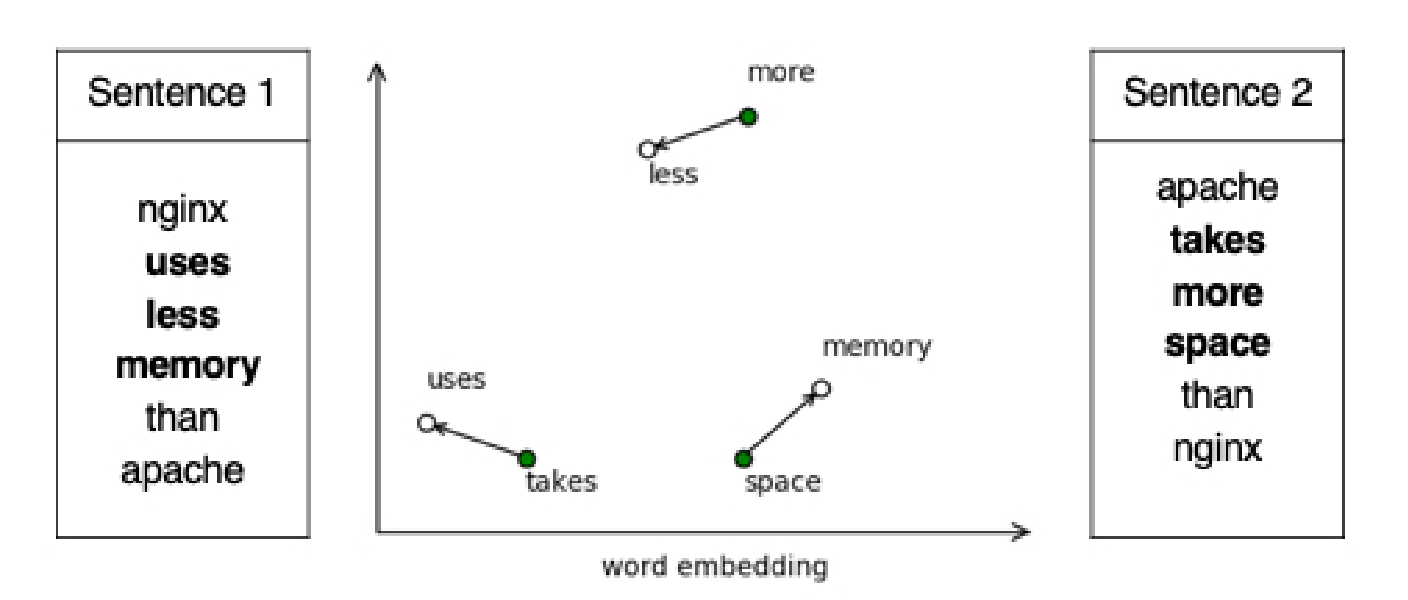
\includegraphics[width=0.49\textwidth]{figures/wmd1.pdf}
	\vspace{-7mm}
	\caption{An illustration of measuring similarity of two comparative sentences \chen{Please use the PDF file.}}
	\vspace{-3mm}
	\label{fig:wmd}
\end{figure}

To use word mover's distance in our approach, we first train a word embedding model based on the post content of Stack Overflow so that we get a dense vector representation for each word in Stack Overflow.
Word embedding has been shown to be able to capture rich semantic and syntactic information of words.
Our approach does not consider word mover's distance for all words in a sentence.
Instead, for each comparative sentence, we extract only keywords with POS tags that are most relevant to the comparison, including adjectives (JJ), comparative adjectives (JJR) and nouns (NN, NNS, NNP and NNPS), not including the technologies under comparison. 
Then, we compute the minimal word movers' distance between the keywords in one sentence and those in the other sentences.
Base on the distance, we further compute the similarity score of the two sentences by 
$$ similarity \ score (S_1, S_2) = \frac{1}{1+D(S_1, S_2)} $$
The similarity score is in range $(0, 1)$, and the higher the score, the more similar the two sentences.
If the similarity score between the two sentences is larger than the threshold, we regard them as similar.
The threshold is 0.55 in this work, determined heuristically by a small-scale pilot study. 
We show some similar comparative sentences by word mover's distance in Table~\ref{tab:wmd}.

To help reader understand word movers' distance, we show an example in Figure~\ref{fig:wmd} with two comparative sentences for comparing \textit{apache} and \textit{nginx}: ``\textit{nginx uses less memory than apache}'' and ``'\textit{Apache takes more space than nginx}'.
The keywords in the two sentences that are most relevant to the comparison are highlighted in bold.
We see that the minimum distance between the two sentences is mainly the accumulation of word distance between pairs of similar words \textit{(uses, takes)}, \textit{(less, more)}, and \textit{(memory, space)}. 
%If we consider the distance between other pairs of words, such as \textit{(security, less)}, \textit{(offer, functionality)}, the overall distance would be much larger.
As the distance between the two sentences is small, the similarity score is high even though the two sentences use rather different words and express the comparison in reverse directions.

\begin{comment}
Word Mover's Distance (WMD) is a novel tool that allows us to accurately measure the similarity between two sentences. As Fig. ~\ref{fig:wmd} shows, apart from the technology names, the two sentences, ``\textit{postgresql} offers more security functionality than \textit{mysql}'' and ``\textit{mysql} provides less safety features than \textit{postgresql}'' have no words in common, but the "traveling distance" between them is small. WMD measures the minimum amount of required distance "moving" from the embedded words of one sentence to the embedded words of another sentence~\cite{kusner2015word}. For normalization, we compute WMD similarity that is simply the negative distance. For each comparative sentence, we use POS tagger to extract adjectives (JJ), comparative adjectives (JJR) and nouns (NN, NNS, NNP and NNPS) as candidate keywords. Then, we calculate WMD similarity based on the four candidate keywords near every technology. 
\end{comment}                                                     

\begin{table*}
	\centering
	\caption{Examples of similar comparative sentences by Word Mover's Distance}
	\vspace{-3mm}
	\begin{tabular}{l|l}
	\hline
	\textbf{Comparable technology pair} & \textbf{Comparative sentences} \\ \hline
	\multirow{2}{*}{\textit{quicksort} \& \textit{mergesort}} & Quicksort is done in place and doesn’t require allocating memory, unlike mergesort. \\ & Mergesort would use more space than quicksort. \\ \hline
	\multirow{2}{*}{\textit{swing} \& \textit{awt}} & Consider using swing which has much better performance over the old heavyweight awt. \\ & Yes swing has newer and better apis than awt. \\ \hline
	\multirow{2}{*}{\textit{google-chrome} \& \textit{safari}} & But safari takes more time than google-chrome browser. \\ &  I get a lot of results about how safari is slower than google-chrome. \\ \hline
	\multirow{2}{*}{\textit{get} \& \textit{post}} & Post is also more secure than get because you aren t sticking". \\ & When you use post data is a a lot more safer than get and you can send large no. of request parameters. \\ \hline
	\multirow{2}{*}{\textit{tcp} \& \textit{udp}} & Tcp is a slower more reliable protocol than udp is. \\ & This is the reason why udp is much faster than tcp. \\ \hline
	\end{tabular}
	\vspace{-1mm}
	\label{tab:wmd}
\end{table*}
	
\subsection{Clustering Representative Comparison Aspects}
For each pair of comparable technologies, we collect a set of comparative sentences about their comparison in Section~\ref{sec:comparativeSentence}.
Within these comparative sentences, we find pairs of similar sentences in Section~\ref{sec:measuresimilarity}.
We take each comparative sentence as one node in the graph.
If the two sentences are determined as similar, we add an edge between them in the graph.
In this way, we obtain a graph of comparative sentences for a given pair of comparative technologies.

\begin{figure}
	\centering
	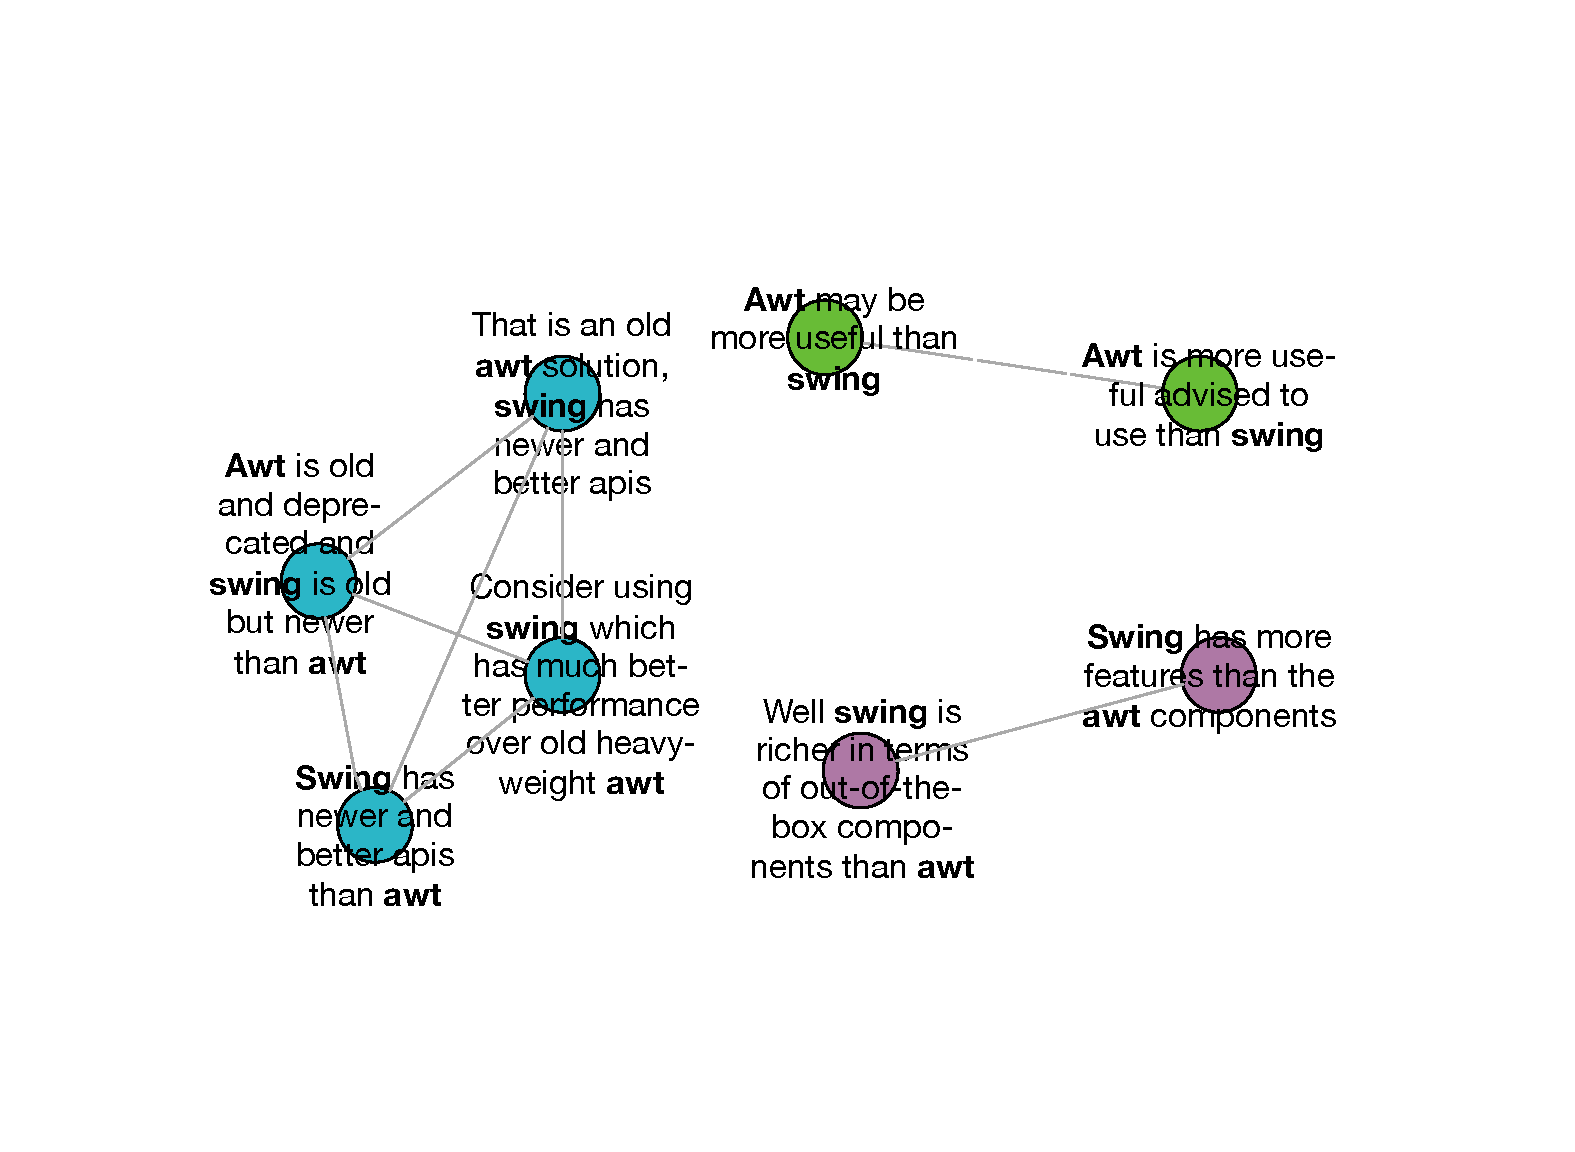
\includegraphics[width=0.45\textwidth]{figures/communities.pdf}
	\vspace{-6mm}
	\caption{Communities in the graph of comparative sentences \chen{This example does not show the power of community detection, as each subgraph is regarded as a community.}}
	\vspace{-3mm}
	\label{fig:communities}
\end{figure} 

Although some comparative sentences are very different in words or comparison directions (examples shown in Fig.~\ref{fig:wmd} and Table~\ref{tab:wmd}), they may still share the same comparison opinions.
In graph theory, a set of highly correlated nodes is referred to as a community (cluster) in the network.
Based on the sentence similarity, we cluster similar opinions by applying the community detection algorithm to the graph of comparative sentences.
In this work, we use the Girvan-Newman algorithm~\cite{girvan2002community} which is a hierarchical community detection method.
It uses an iterative modularity maximization method to partition the network into a finite number of disjoint clusters that will be considered as communities. 
Each node must be assigned to exactly one community.
Fig.~\ref{fig:communities} shows the graph of comparative sentences for the comparison of \textit{awt} and \textit{swing} (two java toolkits), in which each node is a comparative sentence, and the detected communities are visualized in the same color.
%Do we need to introduce the tricks that we use for our cases

As seen in Fig.~\ref{fig:communities}, each community may represent a prominent comparison aspect of the two comparable technologies.
But some communities may contain too many comparative sentences to understand easily.
Therefore, we use TF-IDF (Term Frequency Inverse Document Frequency) to extract keywords from comparative sentence in one community to represent the comparison aspect of this community.
TF-IDF is a statistical measure to evaluate the importance of a word to a document in a collection. 
It consists of two parts: term frequency (TF, the number occurrences of a term in a document) and inverse document frequency (IDF, the logarithm of the total number of documents in the collection divided by the number of documents in the collection that contain the specific term).
For each community, we remove stop words in the sentences, and regard each community as a document.
We take the top-3 words with largest TF-IDF scores as the representative aspect for the community.
Table~\ref{tab:aspects} shows the comparison aspects of four communities for comparing \textit{UDP} with \textit{TCP}.
The representative keywords directly show that the comparison between \textit{UDP} with \textit{TCP} mainly focuses on four aspects: speed, header, usability, and fields that they are used for.

\begin{table*}
	\centering
	\caption{The representative keywords for clusters of \textit{UDP} and \textit{TCP}.}
	\vspace{-3mm}
	\setlength{\tabcolsep}{0.01em}
	\begin{tabular}{l|l}
	\hline
	\textbf{Representative keywords} & \textbf{Comparative sentences} \\ \hline
	\multirow{3}{*}{faster slower reliable} & One often finds the argument that udp is faster then tcp \\ & Udp is way lighter and faster but somewhat less reliable than tcp. \\ & Udp is generally faster than tcp as it does not have to do the overhead checking of consistency that tcp must deal with.\\ \hline
	\multirow{3}{*}{header connection size} & You will notice that the tcp header has more fields than the udp header and many of those fields will be populated. \\ & Udp communication is connection less as compared to tcp which need a connection. \\ & The header size of udp is less than tcp. \\ \hline
	\multirow{3}{*}{harder, easier,travelsal} & Doing p2p nat traversal over tcp is a bit harder than udp. \\ & Keep in mind that implementing udp traversal is easier than tcp. \\ & It was introduced since the nat traversal for tcp is much more complicated than udp. \\ \hline
	%\multirow{3}{*}{better, protocol} & Udp is a lightweight protocol ;tcp is a better choice if you want robust packet delivery and sequencing. \\ & In general the tcp protocol manages the available network bandwidth better than the udp protocol. \\ & Udp scales better than tcp because of reduced states that need to be maintained in the operating system. \\ \hline
	\end{tabular}
	\vspace{-1mm}
	\label{tab:aspects}
\end{table*}


\begin{comment}
If the WMD similarity between comparative sentences exceeds a specified threshold, the two sentences would be added as two nodes and a linking edge to the graph for each similar technology pair. The threshold is not fixed and it depends on the difference between numbers of the extracted keywords. If a comparative sentence was not added to the graph, the sentence would be considered to belong to the ``others'' aspect.
	
After building graph for each similar technology pair, we use Givan-Newman algorithm to detect communities in the graph. The Givan-Newman algorithm is a hierarchical method and hence allows us to control the size of each detected community~\cite{girvan2002community}. We keep the size of communities for each similar technology pair appropriate based on the total number of comparative sentences.

In order to figure out what aspects of technologies users are concerned about, we extract the words with highest TF-IDF values as the aspect for each detected community.

Term frequency-inverse document frequency (TF-IDF) is a statistical measure that is intended to evaluate the importance of a word to a document in a collection. The TF-IDF consists of two parts: term frequency (TF, the number occurrences of a term in a document) and inverse document frequency (IDF, the logarithm of the total number of documents in the collection divided by the number of documents in the collection that contain the specific term). The TF measures the frequency of a term while the IDF reflects the importance of a term. Therefore, the higher TF-IDF value of a term demonstrates that the term is more important to the document.

In our scenario, we utilize the TF-IDF value to extract representative keywords for each clusters. For each comparative technology pair, we consider every cluster as a document and use all documents to form a collection. Then, we calculate the TF-IDF value for each candidate keyword and extract at most three words with highest TF-IDF values as the representative keywords for each cluster.

\end{comment}


\begin{comment}
The main process includes:
\begin{enumerate}
	\item Checking whether a sentence contains similar technology, including checking abbreviations and synonyms.
	\item Labeling all words in a sentence containing similar technology with common POS tags and our extended comparative POS tags;
	\item Using comparative patterns to match the sequence of POS tags. If the sentence matches at least one comparative pattern, we consider it as a comparative sentence.
\end{enumerate}}	

\subsection{Extracting comparative opinions}
By analysing the sentence structure with Natural Language Processing, we extract the comparative relationships (like ``faster''), and relationship direction (like `` java --> python'').
So we transform the unstructured opinions into structured comparison. 

\subsubsection{Relationship extraction}
Observing the identified comparative sentences, we find that most of comparative relationships can be categorized into three patterns of POS tag sequence: RBR JJ (e.g. more powerful), JJR (e.g. faster) and JJR \textit{Noun} (e.g. better performance). Note that \textit{Noun} consists of NN, NNS, NNP and NNPS. We extract the part matching these three patterns in each sentence to represent the comparative relationship between the similar technology included in the sentence.
   
\subsubsection{Topic analysis}
In order to figure out what aspects of technologies users are concerned about, we conduct topic analysis based on the extracted relationships.
We use a keyword-based approach to analyze the topics. The relationships we extracted from comparative sentences are represented by ajectives (JJ), comparative adjectives (JJR) and nouns (NN, NNS, NNP and NNPS). Hence, we compile a list of keywords for each topic as Table 2 shows. The topic of each comparative sentence depends on whether this sentence contains at least one corresponding keyword.

\begin{table*}
	\begin{tabular}{l l l}
		\hline
		Topic \& Adjectives (JJ) & Comparative adjectives (JJR) & Nouns (NN, NNS, NNP \& NNPS) \\ \hline
	\end{tabular}
\end{table*}	


\subsubsection{Preference Analysis} 

\subsection{Organizing the overall comparison}
We need to aggregate all individual opinions into an overview, so that users can obtain a more direct understanding of the different between the similar technology.
\end{comment}